\chapter{Score Matching for Categorical Data via Gumbel Noise }
\label{ch:gnsm}

It is common to represent information as discrete categories such as gender, shapes or product quality.
One may wish to detect anomalies within this data type, in addition to continuous variables. However, MSMA, as it was introduced in the previous chapter is unable to model categorical data.
This is because a score is ill-defined for categorical variables. There is no notion of a gradient for probability density functions~\footnote{In this case, it is more correct to refer to them as probability \textit{mass} function} of discrete data. If we can overcome this limitation, we will be able to incorporate more information into MSMA. Ultimately, my goal is to allow MSMA to model any available metadata that is paired with the continuous features, e.g. demographic data paired with brain MRIs. I posit that this mixed data type modeling would enable more robust anomaly detection decisions.

This chapter introduces Gumbel Noise Score Matching (GNSM), a novel method for learning scores of categorical data for the purpose of anomaly detection.
The chapter first develops the theoretical foundations of GNSM, showing how continuous relaxations of categorical distributions through the Gumbel-Softmax trick can be combined with denoising score matching to estimate scores for categorical variables. The resulting objective allows the model to directly output score estimates for one-hot encoded categorical features. Experiments on a suite of tabular anomaly detection datasets show GNSM-MSMA achieving competitive or state-of-the-art performance compared to baseline methods, with significant improvements on certain datasets. A case study on detecting anomalous image segmentations further illustrates the versatility of the approach beyond just tabular data.

The key contributions of this chapter are: 1) Developing a principled score matching framework for categorical data, and 2) Demonstrating the capability of score matching for anomaly detection on categorical types in both tabular and image datasets. The chapter highlights GNSM as a powerful and flexible approach for handling structured, non-continuous data types in anomaly detection. Related code is available at~\url{https://github.com/ahsanMah/categorical-dsm}

% \smallskip

% Our main contributions are :

% \begin{itemize}
%     \item Deriving an unsupervised training objective for learning the scores of categorical distributions
%     \item Demonstrating the capability of score matching for anomaly detection on categorical types in both tabular and image datasets
%     \item Providing a unified framework for modeling mixed data types via score matching
% \end{itemize} 


\section{A Recipe for Categorical Score Matching}
\label{sec:recipe}

In this section I will develop the ideas behind the GNSM objective. I will start by introducing a technique for continuous approximations (i.e. relaxations) for categorical distributions. I will then formulate an objective (based on denoising score matching) to learn the scores of the relaxed categorical variables. 

\subsection*{Continuous Relaxation to Categorical Data}

Gradients of log likelihoods are ill-defined for categorical inputs. In order to compute the score of categorical data, I propose to adopt a continuous relaxation for discrete random variables co-discovered by~\cite{jang2017categorical, maddison2017concrete}. These relaxations build on the Gumbel-Max trick to sample from a categorical distribution ~\cite{maddison2014sampling}. The procedure (often referred to as the Gumbel-Softmax) works by adding Gumbel noise~\cite{gumbel1954statistical} to the (log) probabilities and then passing the resulting vector through a softmax to retrieve a sharpened probability distribution over the categorical outcomes. Of particular interest to us, Gumbel-Softmax incorporates a temperature parameter ($\lambda$ in Equation~\eqref{eq:log_concrete}) to control the sharpening of the resulting probabilities. I argue that this temperature can also be interpreted as a noise parameter, by virtue of it increasing the entropy of the post-softmax probabilities. I will make use of this intuition to combine continuous relaxations with denoising score matching. 

Note that for the rest of the chapter, I will be utilizing the formulation of~\cite{maddison2017concrete} i.e. concrete random variables. In particular, I will be using a variant of the Concrete Distribution called ExpConcrete introduced by the same authors (shown in~\eqnref{eq:log_concrete}). Given unnormalized probabilities $\alpha \in (0, \infty)^K$, Gumbel i.i.d samples $\mathit{G}_k$, and a smoothing factor $\lambda \in (0, \infty)$, we can construct an ExpConcrete random variable $Y \in \mathbb{R}^n$ such that $\exp(Y) \sim \text{Concrete}(\alpha, \lambda) $:

\begin{equation}
    Y_k = \frac{\log \alpha_k + G_k}{\lambda} - \log \sum_{i=1}^{K} \exp \br{\frac{\log \alpha_i + G_i}{\lambda}}
    \label{eq:log_concrete}
\end{equation}

As $\lambda \rightarrow 0$, the computation approaches an argmax, while large values of $\lambda$ will push the random variable towards a uniform distribution. The main purpose of preferring the ExpConcrete Distribution over the Concrete Distribution is numerical stability, as the former is defined in the log domain.


\subsection*{Score Matching with Categorical Variables}

We now have the basic ingredients to start learning scores for our relaxed-categorical data.
Firstly, note that the proof of the denoising score matching objective by \cite{vincent2011connection} (~\eqnref{eq:denoising_sm}) holds true for any $q_\sigma$, provided that $\log q_{\sigma}(\Tilde{x} |x)$ is differentiable.
Recall that $q_\sigma$ plays the role of a noise distribution. While most denoising score matching models incorporate Gaussian perturbation~\cite{Song2019,song2020score,vincent2011connection}, I emphasize that \textit{any} noise distribution may be used during training.
% \footnote{There are some weak regularity conditions that are almost always satisfied}.

\subsection*{ExpConcrete($\alpha$,~$\lambda$) as a Noise Distribution}
\label{combine}

Following the reasoning above and the temperature parameter ($\lambda$) available in~\eqnref{eq:log_concrete}, I propose to repurpose the Concrete distribution to add `noise' to our continuous relaxations of the categorical variables. Increasing $\lambda$ will allow us to corrupt the input $x$ by scaling the logits and smoothing out the categorical probabilities. Therefore, in GNSM, the (Exp)Concrete Distribution acts both as the relaxation mechanism \textit{and} the noise distribution:

\begin{align*}
     \log q_{\sigma}(\Tilde{\mathbf{x}} | \mathbf{x})  &= \log p_{\lambda}(\Tilde{\mathbf{x}}; \alpha=\mathbf{x})
\end{align*}

Here, the location parameter is that of the unperturbed input (similar to how one would use a Gaussian kernel), and $\lambda$ is a known hyperparameter. I set $\alpha$ to be the logits of $\mathbf{x}$. As $\mathbf{x} \in \br{0,1}^K$ will be a one-hot encoding for $K$ outcomes, it does not strictly satisfy the requirement $\alpha \in (0, \infty)^K$. This can be circumvented by adding a small delta to the vectors to avoid zero values i.e. $\alpha = \mathbf{x} + \delta $. While it is possible to any transformation to convert $\mathbf{x}$ to unnormalized probabilities, I opted to use the clamped one-hot encodings for simplicity.

\subsection*{Score of ExpConcrete Distribution}

To plug ExpConcrete into the DSM objective (\eqnref{eq:denoising_sm}), I first need to derive the the score for the ExpConcrete distribution i.e. take the gradient of the log-density with respect to the data. Conveniently, the authors of ~\cite{maddison2017concrete} derived the log-density of an ExpConcrete random variable, which I will be using going forward:

\begin{equation}
    \label{eq:concrete_log_pdf}
         \log p_{\alpha, \lambda}(x) = \log((K-1)!) + (K-1) \log \lambda~ + \p{ \sum_{k=1}^{K} \log \alpha_k - \lambda x_k } -
         K\log \sum_{k=1}^{K} e^{(\log \alpha_k - \lambda x_k)}
\end{equation}

Here $x \in \mathbb{N} $ such that $ \log \sum_{k=1}^{K} \exp (x) = 0$. Since the first two terms for $\log p_{\alpha, \lambda}(x)$ in~\eqnref{eq:concrete_log_pdf} are independent of $x$, we can ignore them and focus on the latter:

\begin{align}
    \nabla_{x_j} \log p_{\alpha, \lambda}(\mathbf{x}) &= 
    \nabla_{x_j} \p{ \sum_{k=1}^{K} \log \alpha_k - \lambda x_k } -
    \nabla_{x_j} \p{K\log \sum_{k=1}^{K} \exp \br{\log \alpha_k - \lambda x_k} } \\
    &= \nabla_{x_j} \p{ - \sum_{k=1}^{K} \lambda x_k } -
   K \p{ \nabla_{x_j} \log \sum_{k=1}^{K} \exp \br{\log \alpha_k - \lambda x_k}} \\
    &= - \lambda -K\frac{\nabla_{x_j} \p{\sum_{k=1}^{K} \exp \br{\log \alpha_k - \lambda x_k}}}{ \sum_{k=1}^{K} \exp \br{\log \alpha_k - \lambda x_k}} \\
    &= - \lambda -K\frac{\exp \br{\log \alpha_j - \lambda x_j} \nabla_{x_j} (\log \alpha_j - \lambda x_j)}{ \sum_{k=1}^{K} \exp \br{\log \alpha_k - \lambda x_k}} \\
    &= - \lambda -K\frac{\exp \br{\log \alpha_j - \lambda x_j} (- \lambda) }{ \sum_{k=1}^{K} \exp \br{\log \alpha_k - \lambda x_k}} \\
    &= - \lambda + \lambda K~\frac{\exp \br{\log \alpha_j - \lambda x_j}}{ \sum_{k=1}^{K} \exp \br{\log \alpha_k - \lambda x_k}}
\end{align}

Note how the last equation can be rewritten as:
\begin{equation}
\label{eq:concrete_score}
     \nabla_{x_j} \log p_{\alpha, \lambda}(\mathbf{x}) = - \lambda + \lambda K~\sigma(\log \boldsymbol{\alpha} - \lambda \mathbf{x})_j
\end{equation}
where $\sigma(\mathbf{z})_i = \frac{e^{z_i}}{ \sum_{k=1}^{K} e^{z_k}}$ is the softmax function. 

\subsection*{Gumbel-Noise Score Matching Objective}
\eqnref{eq:concrete_score} represents the score function of the ExpConcrete distribution i.e. the gradient of the log-density with respect to the data. We can now combine the ideas from Denoising Score Matching and Concrete random variables.
Combining ~\eqnref{eq:denoising_sm} and~\eqnref{eq:concrete_score}, one obtains

\begin{align*}
\label{eq:cdsm}
    J(\theta) &= \mathbb{E}_{q_{\sigma}} \s{ || s_\theta(x) - \nabla_{\Tilde{x}} \log q(\tilde{x} | x) ||^2 }\\
     &= \mathbb{E}_{p_{\lambda}} \s{ || s_\theta(\Tilde{\mathbf{x}}) - \nabla_{\Tilde{\mathbf{x}}} \log p_\lambda(\tilde{\mathbf{x}} | \mathbf{x}) ||^2 } \\
     &= \mathbb{E}_{p_{\lambda}} \s{ || s_\theta(\Tilde{\mathbf{x}}) - \nabla_{\Tilde{\mathbf{x}}} \log p_\lambda(\tilde{\mathbf{x}} ; \boldsymbol{\alpha} = \mathbf{x}) ||^2 } \\
     &= \mathbb{E}_{p_{\lambda}} \s{ || s_\theta(\Tilde{\mathbf{x}}) - (- \lambda + \lambda K~\sigma(\log \mathbf{x} - \lambda \Tilde{\mathbf{x}})) ||^2 } \\
     &= \mathbb{E}_{p_{\lambda}} \s{ || s_\theta(\Tilde{\mathbf{x}}) - \lambda K~\sigma(\log \mathbf{x} - \lambda \Tilde{\mathbf{x}}))  + \lambda ||^2 } \\
     &= \mathbb{E}_{p_{\lambda}} \s{ || s_\theta(\Tilde{\mathbf{x}}) - \lambda K~\sigma(\epsilon)  + \lambda ||^2 }
\end{align*}

Here $\epsilon=\log \mathbf{x} - \lambda \Tilde{\mathbf{x}}$ and can be loosely interpreted as the ``logit noise" as it is the difference between the original logit probabilities and the perturbed vector. This formulation is analogous to the simplification utilized by \cite{song2020score,ho2020denoising}. It allows me to train the model to estimate the noise directly as the other variables are known constants. Assume a network $\epsilon_\theta$, that takes the input $\Tilde{\mathbf{x}}$. Following ~\eqnref{eq:concrete_score}, I parameterize a score network as $s_\theta(\Tilde{\mathbf{x}})_j = - \lambda + \lambda K~\sigma(\epsilon_\theta(\Tilde{\mathbf{x}}))_j$. I train the network $\epsilon_\theta$ to estimate the noise values $\epsilon$ by the objective below.  

\begin{equation}
\label{eq:train_obj}
    J(\theta)  = \mathbb{E}_{p_{\lambda}} \s{ \lambda^2 K^2 ||( \sigma( \epsilon_\theta(\Tilde{\mathbf{x}}) ) - \sigma(\epsilon) )||^2 }
\end{equation}

Following~\cite{Song2019}, I can modify my loss to train a NCSN with $L$ noise levels i.e. $\lambda \in \br{\lambda_i}_{i=1}^L$:

\begin{equation*}
% \label{ncsn_obj}
    J_{GNSM}(\theta)  = \sum_{i=0}^{L} \lambda_i^2 K^2 ~\mathbb{E}_{\mathbf{x} \sim p_{\text{data}}} \mathbb{E}_{\Tilde{\mathbf{x}} \sim p_{\lambda_i}} \s{ || \sigma( \epsilon_\theta(\Tilde{\mathbf{x}}, \lambda_i) ) - \sigma(\epsilon) ||^2 }
\end{equation*}

Note that our network is now additionally conditioned on the noise level $\lambda$. Finally, our loss objective can be extended to incorporate data with multiple categorical features. For $D$ categories we have:

\begin{equation}
\label{eq:ncsn_obj}
    \sum_{d=0}^{D} \sum_{i=0}^{L} \lambda_i^2 K_d^2 ~\mathbb{E}_{\mathbf{x_d} \sim p_{\text{data}}} \mathbb{E}_{\Tilde{\mathbf{x}}_d \sim p_{\lambda_i}} \s{ || \sigma( \epsilon_\theta(\tilde{\mathbf{x}}_d,  \lambda_i) ) - \sigma(\epsilon)||^2 }
\end{equation}

Here, $K_d$ represents the number of outcomes per category, $x_d$ represents the one-hot vector of length $K_d$, and  $\tilde{\mathbf{x}}_d$ is the continuous, noisy representation of $x_d$ obtained after a Concrete (Gumbel-Softmax) transform.

Thus, I have shown that a Concrete relaxation allows one to model the scores of categorical variables by acting as the noise distribution in the DSM objective. The network will output the scores of the logits representing the categorical feature. Intuitively, these scores are gradients on a simplex which are pointing in the direction of the category that maximizes the likelihood of the datapoint.

\subsection*{A Note on Optimizing the GNSM Objective in Practice}

Observing the loss in ~\eqnref{eq:ncsn_obj}, we see that we are minimizing the difference between two distributions as both inner terms pass through a softmax function. This insight led me to postulate that that one could substitute the mean squared error loss (MSE) for a metric more apt for matching distributions. I therefore ran experiments using the KL divergence objective as shown in \eqref{kl_obj}. This objective showed faster convergence than MSE. Admittedly, this result is only empirical. It may be possible to gain similar improvements in convergence for the MSE by properly tuning the optimization hyperparameters such as the learning rate.

\begin{equation}
\label{kl_obj}
    J_{GNSM}(\theta)  =  \sum_{d=0}^{D} \sum_{i=0}^{L} \lambda_i^2 K_d^2 ~\mathbb{E}_{\mathbf{x} \sim p_{\text{data}}} \mathbb{E}_{\Tilde{\mathbf{x}} \sim p_{\lambda_i}} \s{ D_{\text{KL}} (\sigma(\epsilon) \parallel  \sigma( \epsilon_\theta(\tilde{\mathbf{x}}_d) ) }
\end{equation}


\subsection*{Anomaly Detection via GNSM-based MSMA}
Once a network is trained with the denoising objective in~\eqnref{eq:ncsn_obj}, we can plug the scores into MSMA to identify anomalies. For a given point $x$, I compute the score estimates for all noise perturbation levels. The resulting vector represents the $L$-dimensional multiscale embedding space:
\begin{equation}\label{eq:norms}
    \eta(x) = \left( \norm{  s_\theta(x, \lambda_1) }_2^2, ... , \norm{  s_\theta(x, \lambda_L) }_2^2 \right)
\end{equation}
where $s_\theta(x, \lambda_i)$ is the noise conditioned score network estimating $\nabla_{x} \log p_{\lambda_i}(x)$.
Following the mechanism laid out in Chapter~\ref{ch:msma}, our goal is to learn ``areas of \emph{concentration}" of the inlier data in the $L$-dimensional embedding space ($\eta(x)$, for $x\sim p$). Concretely, I train a GMM on $\eta(X_{\text{IN}})$, where $X_{\text{IN}}$ represents the set of inliers. At inference time, I first use the score network to compute the score-embedding space $\eta(x)$ for the test samples and then compute the likelihoods of the scores via the trained GMM. The negative of this likelihood is then assumed as the anomaly score for the test samples.

\section{What Makes GNSM Appropriate for Anomaly Detection?}
\label{sec:gumbel_ano}

This section will elaborate on the need for GNSM as an anomaly detector. Next, I will demonstrate the use of GNSM combined with MSMA as a promising methodology for anomaly detection in tabular data, which remains an unsolved problem~\cite{pang_deep_2021, ruff_unifying_2021, aggarwal_introduction_2017}.  

\subsection*{Limitations of Current Models in Handling Categorical Data}

The handling of categorical data in anomaly detection has been largely superficial in mainstream methodologies, where only a handful explicitly model categorical data types ~\cite{pang2021homophily}. Recent comprehensive benchmarks, such as the one by~\cite{han2022adbench}, reveal a notable gap: none of the tested methods utilize categorical data's intrinsic properties. Traditional approaches convert categorical variables into one-hot or binary encodings, subsequently treating them as if they were independent, continuous variables. This representation is fundamentally flawed as it ignores the exclusive nature of categorical variables, where the presence of one class implicitly denotes the absence of others within the same category.

This oversight in existing models highlights a significant opportunity for advancement. Drawing a parallel from the evolution in deep learning for computer vision, the success of seminal convolutional neural networks such as ~\cite{alexnet,vgg} is attributed to their inductive bias – the assumption that neighboring pixels in an image are correlated. This understanding led to the development of convolutional kernels, which are well-suited for image data.

In a similar vein, for categorical data, a more fitting approach is to model each category as a probability distribution, acknowledging the inherent dependence among classes within a category. While classes within a category are dependent, it is reasonable to consider different categories as independent.

GNSM addresses this gap by treating each categorical variable distinctly. Internally, it employs a Gumbel-Softmax relaxation for each one-hot encoded vector. The model computes loss on a per-category basis, thereby respecting and leveraging the inter-class dependencies within each category. This design choice reflects a significant inductive bias of GNSM, aligning closely with the inherent structure of categorical data.  Furthermore, GNSM yields a straightforward approach to model mixed continuous/discrete features via estimating scores through a denoising objective..

%  None of the methods tested in the recent comprehensive benchmark performed by~\cite{han2022adbench} make explicit use of categorical information. After transforming the categorical variables into one-hot or binary encodings, existing methods proceed to treat them as independent (continuous) variables. In reality, each categorical variable can only be one class at a time. Therefore, these models make an incorrect assumption by foregoing the dependence between classes within a category. 

% This leaves room for improvement for constructing a model that is more directly suited to the data type. Recall that the success of recent deep learning computer vision models came in the form of convolutional networks\cite{alexnet,vgg}. It is not by accident that these models carry a strong inductive bias about the data i.e neighbouring pixels in an image are highly likely to be correlated. Therefore, convolutional kernels are an appropriate mechanism for modeling images. 

% Similarly, I argue that we may improve performance by using a model with an inductive bias appropriate to categorical data. Practically, this means that each one-hot encoding of a category should be modeled as a probability distribution i.e. there exists a dependence between classes of a category. Of course, one-hot vectors for different categories may be modeled as independent of each other.

% GNSM enforces this inter-class dependence by modeling each  categorical variable separately. Every one-hot vector undergoes its own Gumbel-Softmax relaxation and the loss is computed per-category. I believe this inductive bias to be a strong asset of GNSM.

\subsection*{Most Anomaly Detection Methods Require Labels}

There is a dearth of unsupervised deep learning anomaly detection methods that excel on tabular datasets. For example, the otherwise exhaustive benchmark of~\cite{han2022adbench} reports only two unsupervised deep learning models, DSVDD \cite{pmlr-v80-ruff18a} and DAGMM \cite{zong2018deep}, in their analysis; with both models being outperformed by shallow unsupervised methods. Some reconstruction-based autoencoder approaches have been proposed~\cite{hawkins2002outlier} but they require optimization tricks such as adaptive sampling, pretraining, and ensembling to work effectively~\cite{chen2017outlier}. 
GNSM, combined with MSMA, offers a straightforward approach to model the data characteristics (i.e. the scores) and detect anomalies. Therefore, I argue that GNSM is a noteworthy addition to the class of unsupervised anomaly detection methods.

\subsection*{GNSM Advances Categorical Score Matching: Denoising and Beyond}

Finally, I emphasize that my method introduces a streamlined approach to estimate scores for categorical data using denoising score matching. Recently, \cite{sun2023scorebased} proposed a ratio matching objective, which may be viewed as a discrete analogue to score matching with continuous variables. However, this method mandates the parameterization of conditional densities, necessitating a crafted architecture to mask specific input segments. In contrast, my method sidesteps such complexities, and can fit into any established score matching framework. For example, my method is compatible with alternative (non-denoising) score matching objectives such as sliced-score matching \cite{song2020sliced}, or the implicit score matching objective originally proposed by \cite{hyvarinen2005}.

Further, there exists a link between score matching and diffusion models as established by \cite{song2020score}. Indeed, recent works such as \cite{structured, argmax} model categorical distributions through a diffusion process. However, it is important to note that these generative models eschew the estimation of the score function $s(x) = \nabla_x \log p(x)$ . Instead, they incorporate the Markov chain interpretation of diffusion models, and directly predict the parameters for transition kernels. As a consequence, these models are not directly suitable for a spectrum of score-based applications, such as out-of-distribution detection as explored in my research, or hypothesis testing as introduced by \cite{hypothesis}. It is plausible that forthcoming research will unveil further applications of score functions, wherein our methodology stands ready to extend these findings to categorical data. 

\section{Experiments on Tabular Benchmark Datasets}\label{sec:gnsm_experiments}

This section will quantitatively assess the performance of GNSM compared to baselines. I created an experimental testbed featuring categorical anomaly detection datasets sourced from a publicly available curated repository\footnote{\scriptsize https://sites.google.com/site/gspangsite/sourcecode/categoricaldata}. Note that for my method, I need to know the number of outcomes for each category to appropriately compute the softmax over all classes. This requirement prevents me from using preprocessed datasets, such as those made available by ~\cite{han2022adbench}. It is also the reason why I could not use all the datasets in the curated repository, as some had been pre-binarized and do not provide further details about the number of classes.

The collected datasets are first split into inliers and outliers. Next, I divided the inliers into an 80/10/10 split for train, validation, and test respectively. The validation set is used for early stopping and the checkpoint with the best validation loss is used for inference. The test set is combined with the outliers and used for assessing performance. The categorical features were first converted to one-hot vectors and then passed through a log transform to retrieve logits. I used standard normalization to normalize any continuous features (only relevant for Census). I report detection performance across five runs with different seeds.

\begin{table}
    \centering
    \small
    \begin{tabular}{rccc}
      \toprule % from booktabs package
      \bfseries Dataset & \bfseries \# Samples & \bfseries \# Anomalies & \bfseries \# Features \\
      \midrule 
      Bank & 36548 & 4640 & 53 \\
      Census & 280717 & 18568 & 396 (+5 cont.)\\
      Chess & 28029 & 27 & 40 \\
      CMC & 1444 & 29 & 25 \\
      Probe & 60593 & 4166 & 67 \\
      Solar & 1023 & 43 & 41 \\
      U2R & 60593 & 228 & 40 \\
      Nursery & 4648 & 328 & 26 \\
      \bottomrule
    \end{tabular}
    \caption{Statistics of public tabular datasets commonly used for evaluating anomaly detectors. All datasets other than Census are categorical only.}\label{tab:data}
\end{table}

I chose four methods to represent baseline performance in lieu of a comprehensive analysis with multiple methods. I was inspired to go this route due to the thorough results reported by ADBench~\cite{han2022adbench}. As the authors describe, no one method outperforms the rest. I picked two representatives for shallow unsupervised methods: Isolation Forests and ECOD. I picked these as they consistently give good performance across different datasets and require little to no hyper parameter tuning. There are much fewer options for unsupervised deep learning methods that have been shown to work on tabular datasets. I chose two models that are popular in this field: DAGMM and DSVDD. Note that these were the only unsupervised deep learning models reported by ~\cite{han2022adbench}.

For my score network, I used a ResNet-like architecture inspired by~\cite{gorishniy2021revisiting}. I replaced \texttt{BatchNorm} layers with \texttt{LayerNorm} and set \texttt{Dropout} to zero. The dimensions of the \texttt{Linear} layers in each block were set to 1024. All activations were set to \texttt{GELU}(~\cite{gelu}) except for the final layer, which was set to \texttt{LeakyReLU}. The number of residual blocks was set to 20. 
To condition the model on the noise scales, I added a noise embedding layer similar to those used in diffusion models \cite{song2020score}. I used the same architecture across all datasets.

My noise parameter $\lambda$ is a geometric sequence from $\lambda=2$ to $\lambda=20$. Early testing showed that the models gave numerical issues for values lower than 2. For the upper-limit (i.e. the largest noise scale) we chose 20 as it works well to smooth out the probabilities to uniform across all datasets. We set the number of noise scales ($L$) to 20. We compute the score norms on the inliers (train+val) according to ~\ref{eq:norms} and train a GMM on the resulting features. The negative likelihoods computed from the GMM are the final outputs of my method.

\subsection*{Results}

\begin{table*}[!ht]
    \centering
    \small
    \hspace*{-0.8cm}\begin{tabular}{c|c|ccccc}
    Dataset & Ano Ratio & IForests       & ECOD           & DAGMM          & DSVDD          & GNSM (Ours) \\
    \midrule
    Bank   & 0.56 & 63.24 $\pm$~1.74 & \textbf{66.52 $\pm$~0.57} & 57.62 $\pm$~3.36 & 58.50 $\pm$~5.30 & 65.58 $\pm$~3.45 \\
    Census  & 0.40 & 40.64 $\pm$~2.07 & 40.96 $\pm$~0.15 & 32.90 $\pm$~5.00 & 41.18 $\pm$~3.44 & \textbf{47.79 $\pm$~2.29} \\
    Chess   & 0.01 & \textbf{2.31 $\pm$~1.36} & 1.43 $\pm$~0.05 & 1.08 $\pm$~0.44 & 1.47 $\pm$~0.54 & 1.60 $\pm$~0.68  \\
    CMC      & 0.17 & 22.72 $\pm$~1.57 & 23.79 $\pm$~1.75 & 24.99 $\pm$~5.75 & 21.99 $\pm$~6.15 & \textbf{25.87 $\pm$~9.93} \\
    Probe    & 0.41 & 92.95 $\pm$~2.28 & 95.39 $\pm$~0.38 & 66.40 $\pm$~9.43 & 89.16 $\pm$~8.40 & \textbf{97.48 $\pm$~0.62} \\
    Solar   & 0.30 & 67.99 $\pm$~3.48 & \textbf{72.23 $\pm$~0.91} & 50.84 $\pm$~5.19 & 51.21 $\pm$~3.94 & 69.28 $\pm$~1.96 \\
    U2R     & 0.04 & 52.74 $\pm$~12.88 & 67.84 $\pm$~1.39 & 10.06 $\pm$~6.47 & 71.17 $\pm$~24.65 & \textbf{82.35 $\pm$~5.45} \\
    Nursery & 0.43 & 46.51 $\pm$~6.52 & \textbf{100.00 $\pm$~0.00} & 48.33 $\pm$~8.64 & \textbf{100.00 $\pm$~0.00} & \textbf{100.00 $\pm$~0.01} \\
    \midrule
Average & - & 48.64 $\pm$ 3.99 & 58.52 $\pm$ 0.74 & 36.52 $\pm$ 5.53 & 54.33 $\pm$ 7.49 & \textbf{61.24 $\pm$ 3.05}
    % \bottomrule
    \end{tabular}
    \caption{Average Precision across multiple datasets. Higher is better. Each experiment was repeated with 5 different seeds and we report the mean and standard deviations across seeds. IForest and ECOD represent shallow models, while DAGMM and DSVDD represent deep learning models. Ano ratio refers to the ratio of anomalies in the test set.}
    \label{tabular_results}
\end{table*}

Table~\ref{tabular_results} reports the Average Precision error (AP) which can also be interpreted as the Area Under the Precision Recall curve (AUPR).  Average precision computes the mean precision over all possible detection thresholds. I chose to highlight AP over AUROC as it is a more apt measure for detecting anomalies, where one often has unbalanced classes. Additionally, precision measures the positive predictive value of a classification i.e. the true positive rate. This is a particularly informative measure for anomaly detection algorithms where one is preferentially interested in the performance over one class (outliers) than the other (inliers). I would also like to note that the anomaly ratios in the test set do not correspond with the true anomaly ratio in the original dataset. This is due to my data splitting scheme where my test set is effectively only 10\% the size of inliers.

Table~\ref{tabular_results} shows that GNSM-based MSMA performs better or on par with baselines. GNSM achieves significant performance improvements over baselines for Census, Probe and U2R, respectively achieving a 6.61\%, 2.09\%, and 11.18\% improvement over the next best method respectively.

Results for CMC and Bank are less straightforward to interpret as the differences in the models are not statistically significant, made apparent by the large overlap in the standard deviations. This is especially true for deep learning models which have to be optimized via gradient descent. On Solar, ECOD outperforms the rest by a significant margin. However, among the deep learning models, GNSM performs notably better. Note that Solar is the smallest dataset in this benchmark, with less than 800 training samples.

Lastly, every model struggled with Chess, quite possibly due to the exceptionally small anomaly ratio. While Isolation Forests achieves the highest mean, it is uncertain whether the win is statistically significant. One could easily opt in favor of the other methods for this dataset as they achieve more consistent results. Again, among deep learning models, GNSM performs better.

Overall, we observe that shallow models give more stable and consistent results, with ECOD having the smallest standard deviations on average. Additionally, note that all algorithms struggle on this benchmark. This behavior is prevalent in the field of unsupervised anomaly detection methods, where models exhibit a large variance in accuracy across datasets \cite{han2022adbench}.
As such, in my testing, no one method definitively outperforms the rest; an outcome that coincides with previous findings of~\cite{han2022adbench, pang_deep_2021, ruff_unifying_2021}.

In this context, I emphasize that GNSM consistently ranks high across all datasets tested. In contrast, each of the competing methods were the top performer in only one of the datasets in Table~\ref{tabular_results}, and significantly underperformed in others. Averaged over all datasets, GNSM performs best. This is empirical confirmation that GNSM is a consistent contender in the suite of available algorithms for practitioners looking to detect anomalies in unlabeled data domains.

\section{Case Study: Detecting Segmentation Failures}
\label{sec:cat-seg-study}
I designed this case study to demonstrate how GNSM may be applied to a real world use case of detecting anomalous segmentation masks.
The task here is to learn the distribution of ground truth image-segmentation pairs. At inference time, GNSM-MSMA will score the outputs of a pretrained segmentation model. My hypothesis is that GNSM will correctly detect failure cases i.e. poor segmentations will be ranked higher on the anomaly scale.

While there are many ways to qualitatively define a failure, I will be using popular segmentation metrics (with respect to ground truth masks) as a proxy for performance. I posit that a useful anomaly score should correlate meaningfully with the ground truth segmentation accuracies. 

I compare the anomaly scores against three common segmentation metrics: the Dice similarity coefficient (Dice), the mean surface distance (MSD), and the 95-th percentile Hausdorff distance (95-HD). I chose Dice as it is a popular segmentation metric that measures the overlap between the predicted masks and the ground truth. However, as Dice scores may overestimate performance, it is recommended to additionally report distance based metrics~\cite{valentini2014recommendations, taha2015metrics}. These metrics compute the distance between the surfaces of the predictions and ground truth masks.

I train a convolutional noise conditioned score network on the train-set of the Pascal-VOC segmentation dataset ~\cite{Everingham10}. The model takes in a pairs of images and the one-hot segmentation masks. The model predicts the scores for the segmentation masks only. I chose to use paired data rather than segmentations alone as I want the model to learn whether a segmentation is appropriate for the \textit{given} image. 

As my test subject, I retrieved a pretrained \texttt{DeepLabV3 MobileNet (V3 Large)} segmentation model~\cite{chen2017rethinking} from the publicly available PyTorch implementation ~\footnote{\tiny \text{https://pytorch.org/vision/stable//models/deeplabv3.html}}. This model was trained on a subset of the COCO dataset~\cite{cocodataset}, using only the 20 categories that are present in the Pascal VOC dataset. I used the validation set of Pascal VOC as the test set.

I compare the performance of GNSM to a convolutional DSVDD~\cite{pmlr-v80-ruff18a}. While there may exist specialized segmentation uncertainty estimators, I argue that an unsupervised model provides a more apt comparison. It is reasonable to postulate that both GNSM and DSVDD could be improved by additionally incorporating segmentation-specific objectives into the training, but that remains outside the scope of this study. 

For my score matching network, I adopted the NCSN++ model used by~\cite{song2020score}. The only significant change was in the input/output layers as I am predicting scores over one-hot segmentation masks. For DSVDD, I used the implementation of the original authors~\cite{pmlr-v80-ruff18a}. To keep a fair comparison, we modified the code to use a modern architecture as the backbone (specifically EfficentNetV2~\cite{tan2021efficientnetv2}) and kept the number of parameters similar to our model. Both models were trained to convergence and the best checkpoints (tested over a validation split of the train-set) were used for the analysis.

\subsection*{Detection Results}
\label{seg_results}

\begin{figure}[htbp]
  \centering
  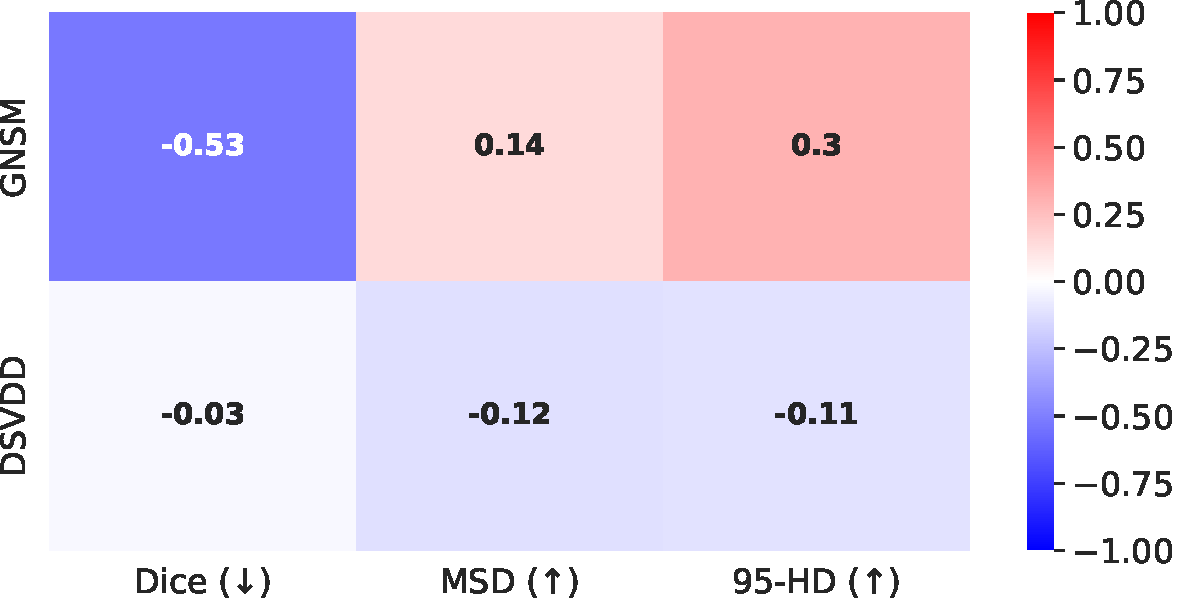
\includegraphics[width=0.7\columnwidth]{figures/voc_heatmap.pdf}
  \caption{Correlations with segmentation metrics for Top-$K=50$ anomaly scores retrieved from GNSM and Deep SVDD. The arrows next to the metric denote the expected correlation direction. The magnitude of the correlations reflects how well the anomaly scores capture segmentation errors.}
\label{corrs}
\end{figure}


\begin{figure*}[htbp!]
  \centering
  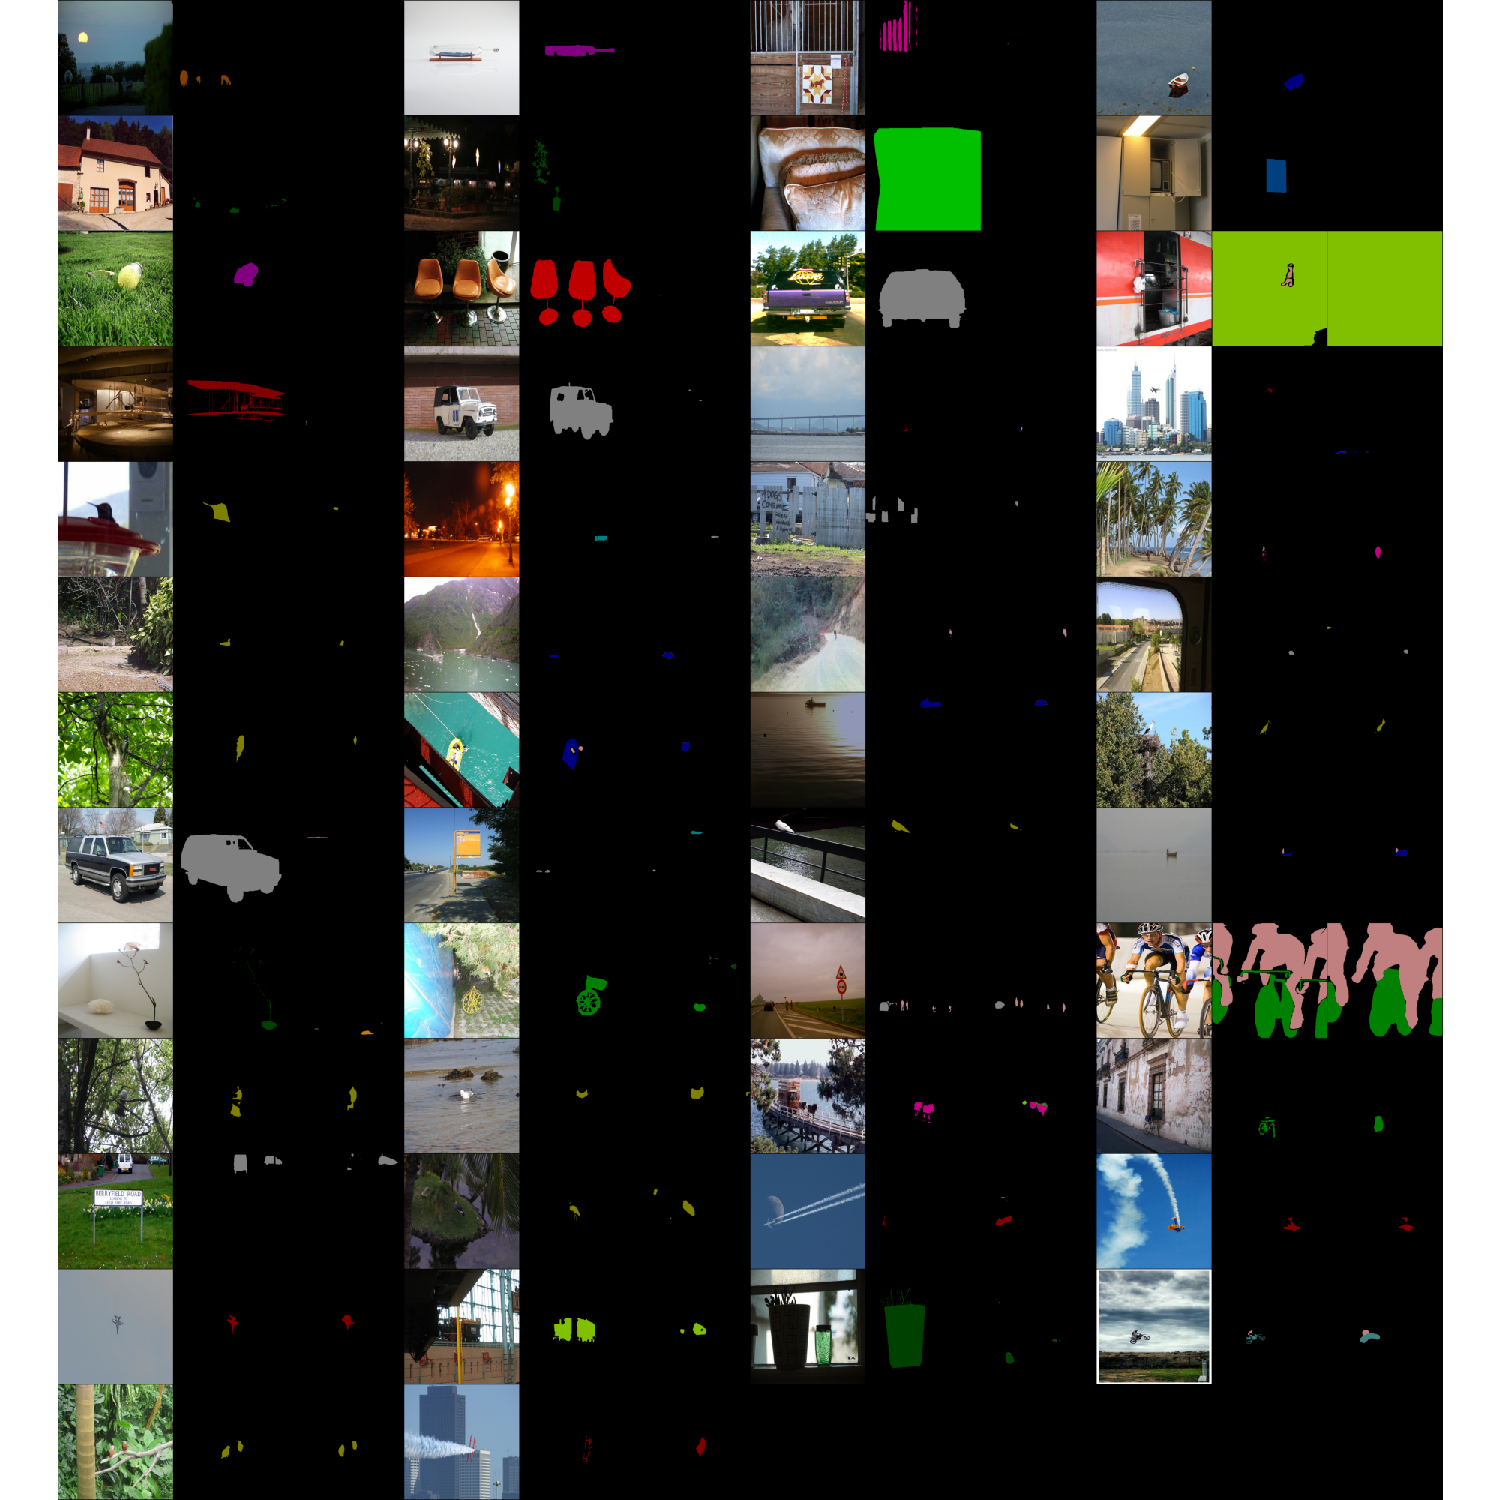
\includegraphics[width=\textwidth]{figures/msma_k50_samples_s.pdf}
  \caption{Samples from Top-K=50 GNSM rankings. The columns (repeated) show input image, ground truth segmentations, and model predictions respectively.  }
  % \label{fig:msma_samples_k50}
  \label{fig:gnsm_samples}
\end{figure*}

\begin{figure*}[htbp!]
  \centering
  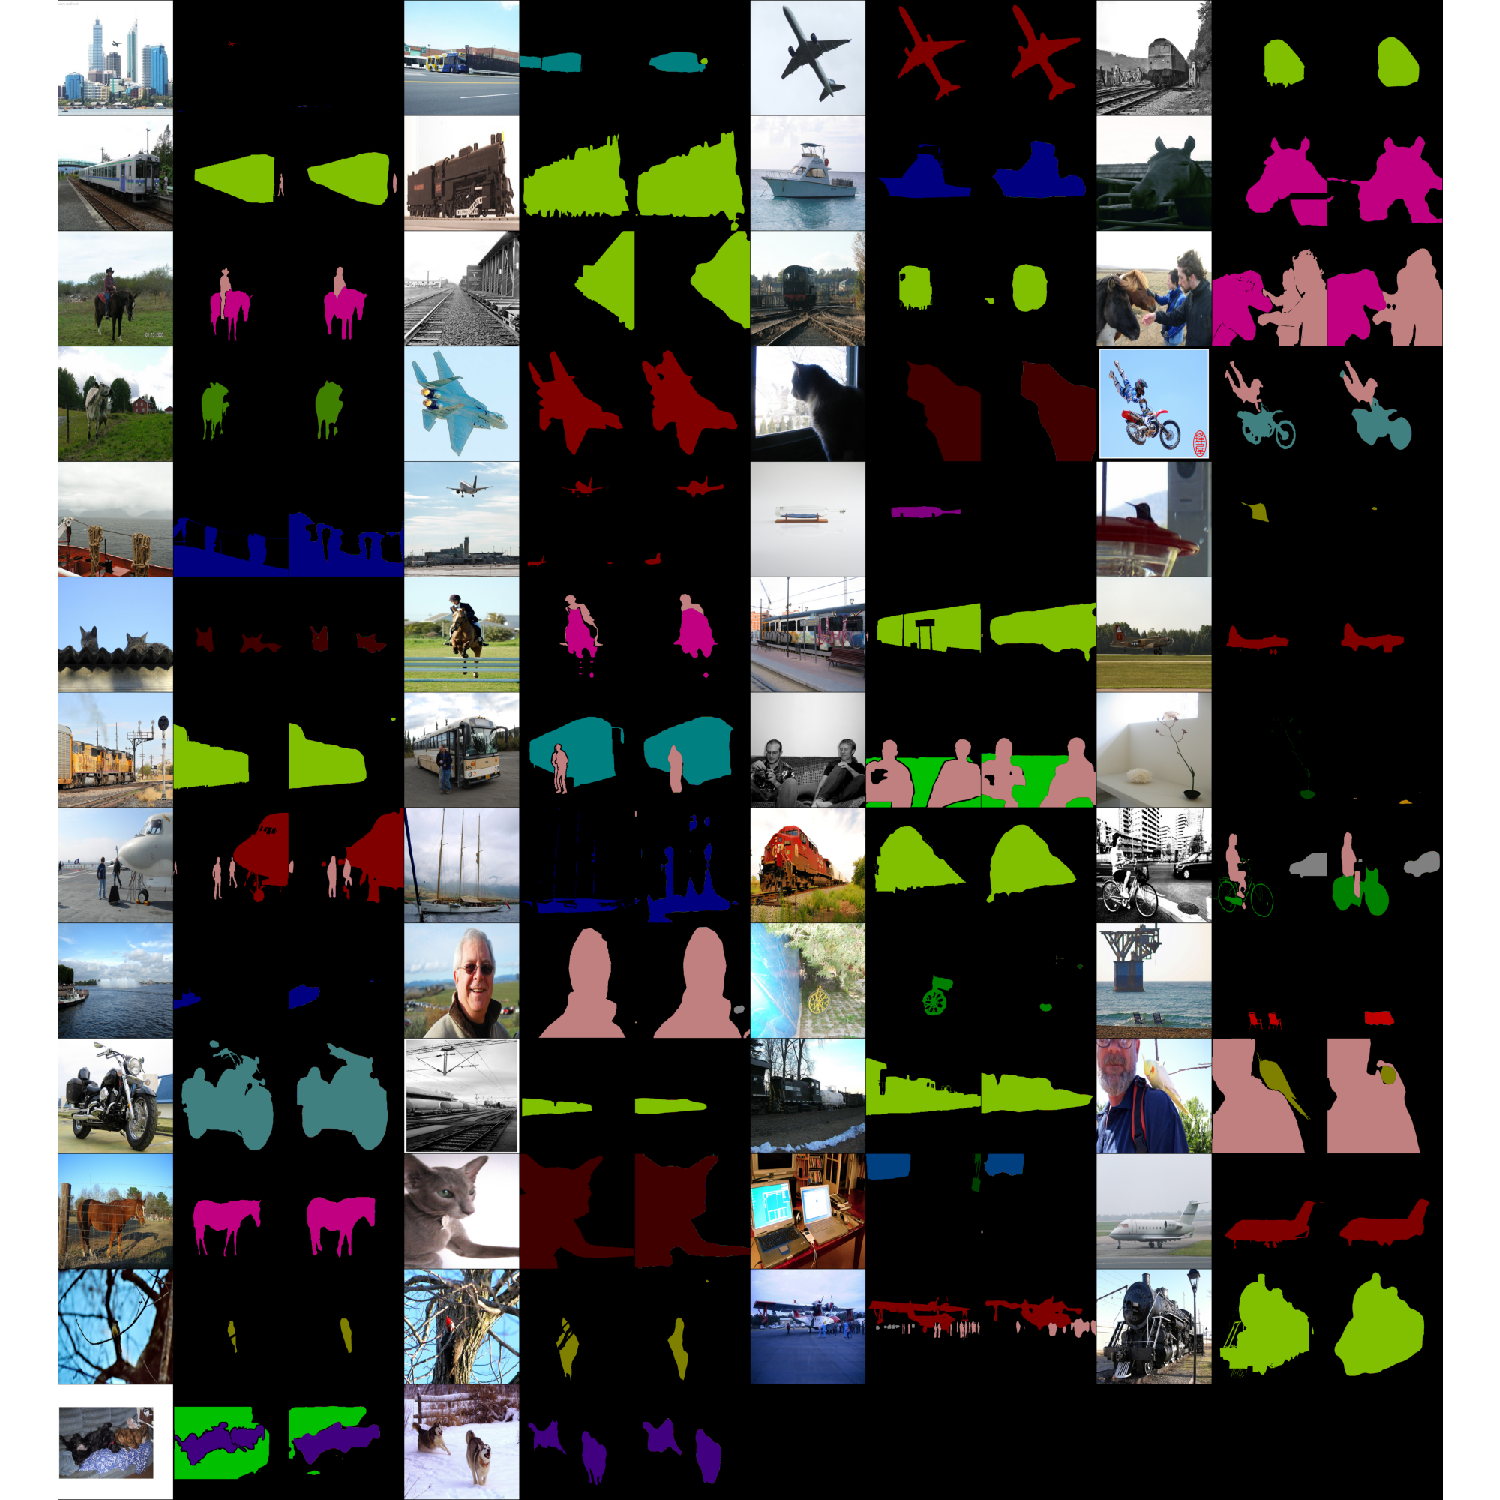
\includegraphics[width=\textwidth]{figures/dsvdd_k50_samples_s.pdf}
  \caption{Random samples from Top-K=50 DSVDD rankings. The columns (repeated) show input image, ground truth segmentations, and model predictions respectively.  }
  % \label{fig:dsvdd_samples_k50}
  \label{fig:dsvdd_samples}
\end{figure*}


% \begin{figure*}\label{fig:samples}
%      \begin{subfigure}[t]{0.92\textwidth}
%          \centering
%         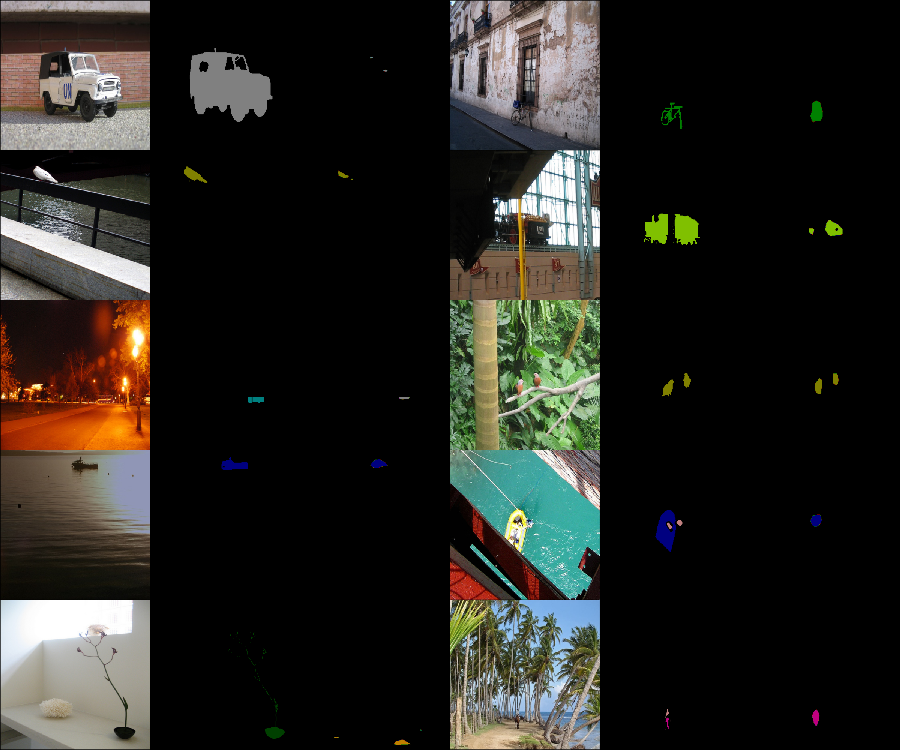
\includegraphics[width=0.95\textwidth, height=4.2in]{figures/msma_rand_samples_s.pdf}
%       \caption{Random samples from Top-K=50 GNSM rankings. Note how the predicted segmentations are either partial/missing or include incorrect classes.}
%       \label{fig:gnsm_samples}
%      \end{subfigure}

%      \begin{subfigure}[t]{0.92\textwidth}
%          \centering
%          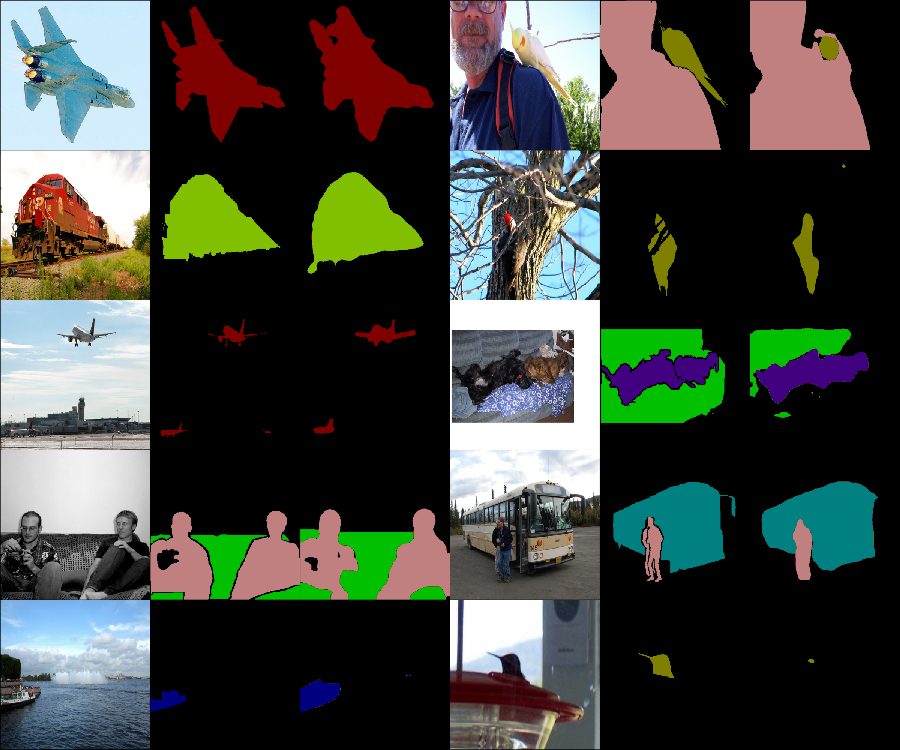
\includegraphics[width=0.95\textwidth, height=4.2in]{figures/dsvdd_rand_samples_s.pdf}
%          \caption{Random samples from Top-K=50 DSVDD rankings. Note how only a few predictions may be considered anomalous.}
%          \label{fig:dsvdd_samples}
%      \end{subfigure}
% \caption{Random samples from Top-K=50 anomaly rankings. The columns (repeated twice) show input image, ground truth segmentations, and model predictions respectively. Different classes are denoted by color.}
% \end{figure*}

I computed the anomaly scores from both GNSM and DSVDD and ranked the images from most to least anomalous. Next, I took the top $K=50$ images (out of 1449) and computed the  Pearson correlation coefficients between the ground truth segmentation metrics and the anomaly scores. I chose the worst ranked images for our analysis as we are interested in the efficacy of these scores for identifying segmentation failures as opposed to assessing the quality of successful segmentations.

Figure~\ref{corrs} shows the correlations between the ground truth segmentation metrics and the anomaly scores from GNSM and DSVDD.  Recall that Dice is a similarity metric while MSD and 95-HD are both distance-based metrics. Therefore, I initially hypothesized that a good anomaly score should correlate negatively with Dice and positively with the distances. Our results show that GNSM correlates strongly in the direction expected. DSVDD on the other hand achieved a poor correlation with Dice and inverse correlations with the distance based metrics.

To qualitatively assess the results of each model a subset of the worst ranked predictions are plotted alongside the groundtruth in Figures~\ref{fig:gnsm_samples},\ref{fig:dsvdd_samples}.
The figures show predictions that were ranked to be anomalous by GNSM~\ref{fig:gnsm_samples} and DSVDD~\ref{fig:dsvdd_samples}. Images are displayed in order from highest ranking to lowest (displayed left to right).

Observe how the predictions ranked by GNSM in Figure~\ref{fig:gnsm_samples} are either complete failures (most of the image is designated the background class) or severe under-segmentations. Predictions ranked by DSVDD in Figure~\ref{fig:dsvdd_samples} do not exhibit any obvious pattern of segmentation failures, with most being reasonable predictions.
% Please look at the extended results in Section~\ref{gnsm_ext_res} for all sorted $K=50$ rankings. 


I believe these results not only exemplify GNSM’s generalization capabilities to non-tabular data, but also highlight a practical application. Quantifying segmentation uncertainties is useful when deploying off-the-shelf models. My experiments prove that GNSM-MSMA may be employed as a filtering mechanism to automatically detect poor segmentations, which could then be reviewed further downstream.

\section{Limitations}

Early testing showed that my score networks need to be deep and require more parameters than baselines. Although my proposed network size is performant, I observed a trend of increased performance as the models got deeper and wider. Due to time and resource constraints, I could not thoroughly explored the architecture space. Additionally, my models take a significant number of iterations to converge. For my experiments, I trained for 1 million iterations, which can take up to a day of training. This is admittedly in contrast to the baselines which may take a few seconds for shallow models and up to a few hours for the deep learning models.

I also acknowledge that GNSM explicitly needs to know the number of outcomes per category to appropriately add noise and compute the scores. While this is a strength of my approach, it does make for an overhead on the user's part. The baselines do not require this additional modeling complexity and are more straightforward to apply. Lastly, my method has hyperparameters pertaining to noise such as the number of scales used and the range of noise levels. While GNSM's hyperparameters have been proven to be stable, I posit that additional improvements may be obtained if these were also tuned per dataset.


\section{Conclusion}

This chapter introduced Gumbel Noise Score Matching (GNSM): a novel method for learning scores of categorical data types. Section~\ref{sec:recipe} outlines how to compute scores of continuously relaxed categorical data and derive the appropriate training objective based on denoising score matching. Section~\ref{sec:gumbel_ano} demonstrates how the estimated scores could be used for anomaly detection when plugged into MSMA.

GNSM achieves competitive performance with respect to baselines on a suite of tabular anomaly detection datasets, attaining significant improvements on certain datasets. Furthermore, GNSM can easily be extended to images and excels on the real-world task of detecting anomalous segmentations, as highlighted in Section~\ref{sec:cat-seg-study}. Lastly, I believe this categorical score matching formulation could be incorporated into generative models. I hope this direction may be explored in future work.

% \section{Extended Results}\label{gnsm_ext_res}

% Here I am displaying show the predictions that were ranked to be anomalous by GNSM~\ref{fig:msma_samples_k50} and DSVDD~\ref{fig:dsvdd_samples_k50}. Images are displayed in order from highest ranking to lowest (displayed left to right).

% \begin{figure*}[htbp!]
%   \centering
%   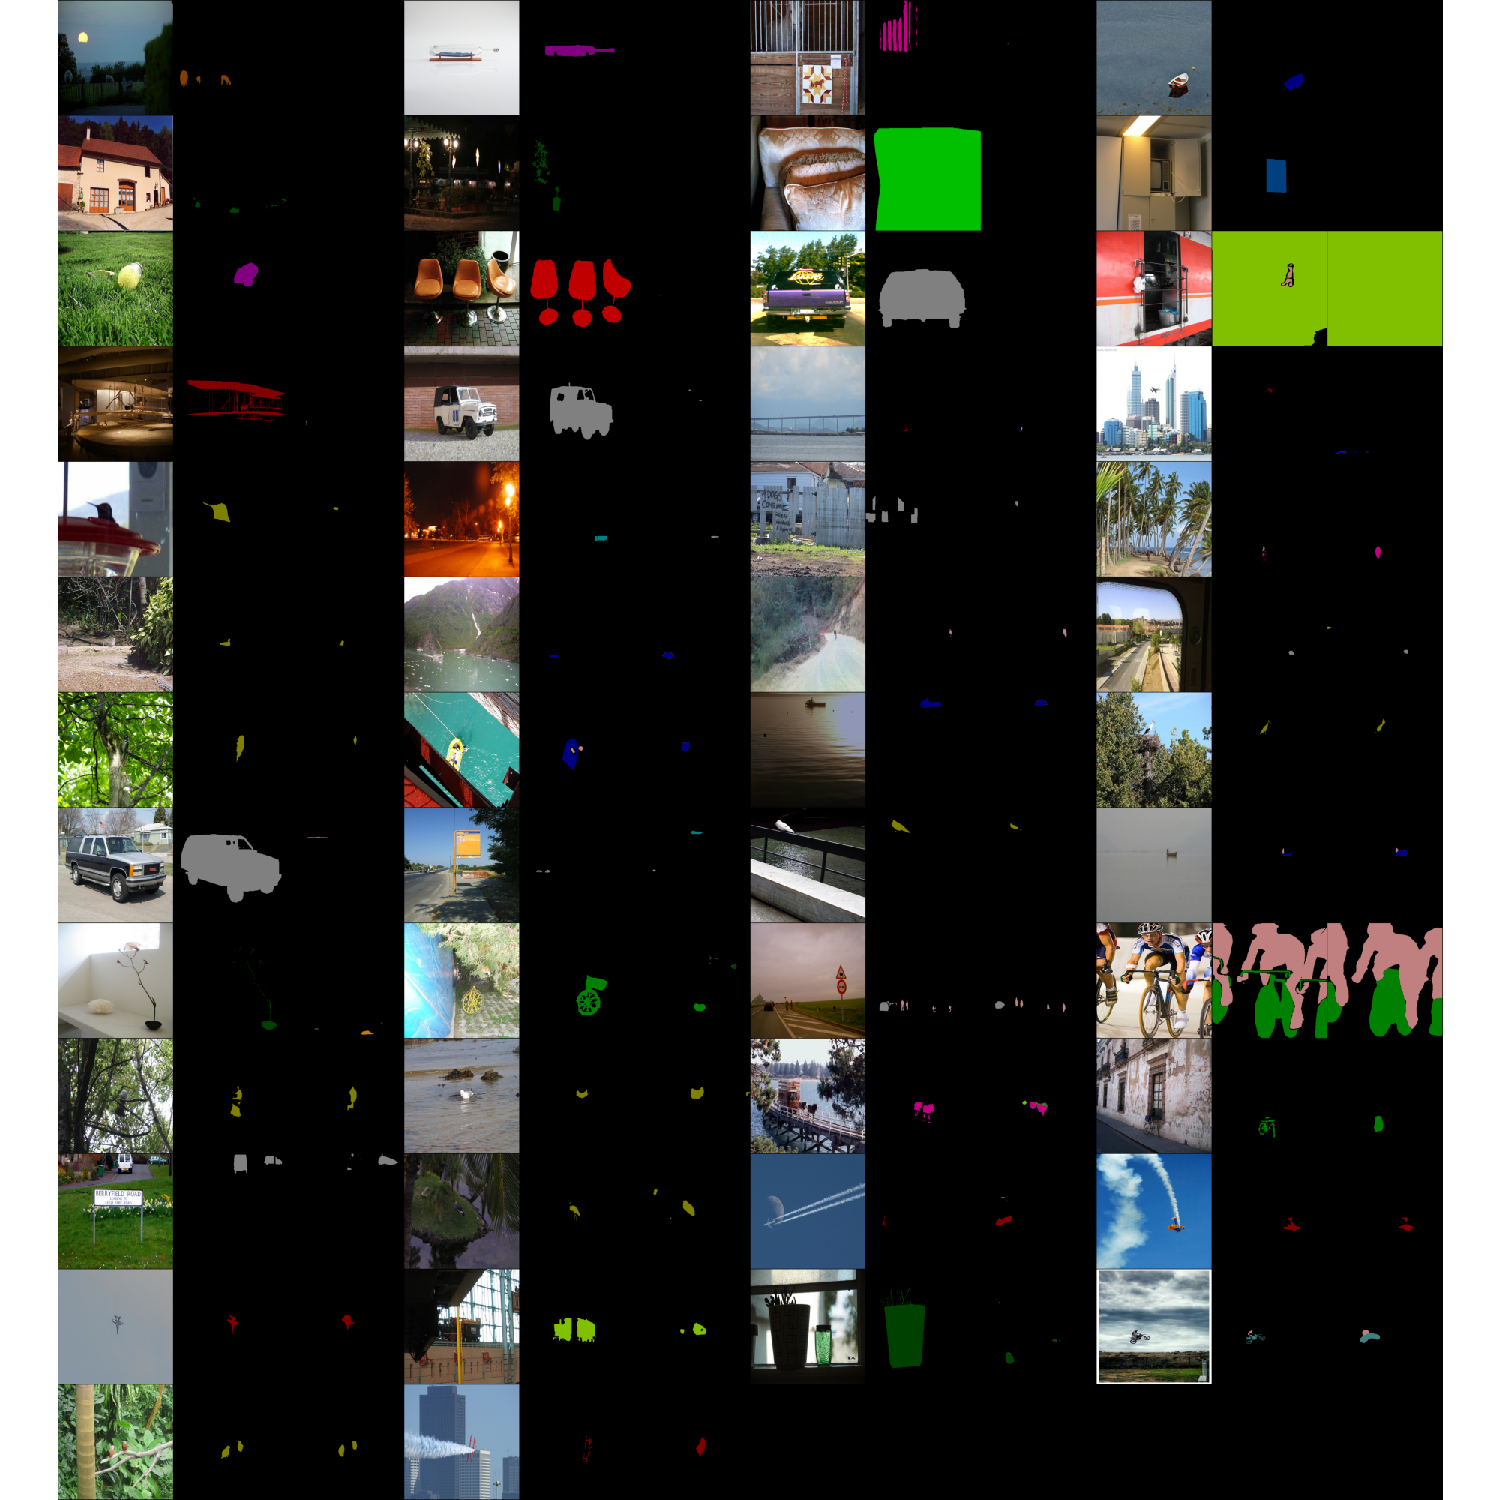
\includegraphics[width=\textwidth]{figures/msma_k50_samples_s.pdf}
%   \caption{Samples from Top-K=50 GNSM rankings. The columns (repeated) show input image, ground truth segmentations, and model predictions respectively.  }\label{fig:msma_samples_k50}
% \end{figure*}

% \begin{figure*}[htbp!]
%   \centering
%   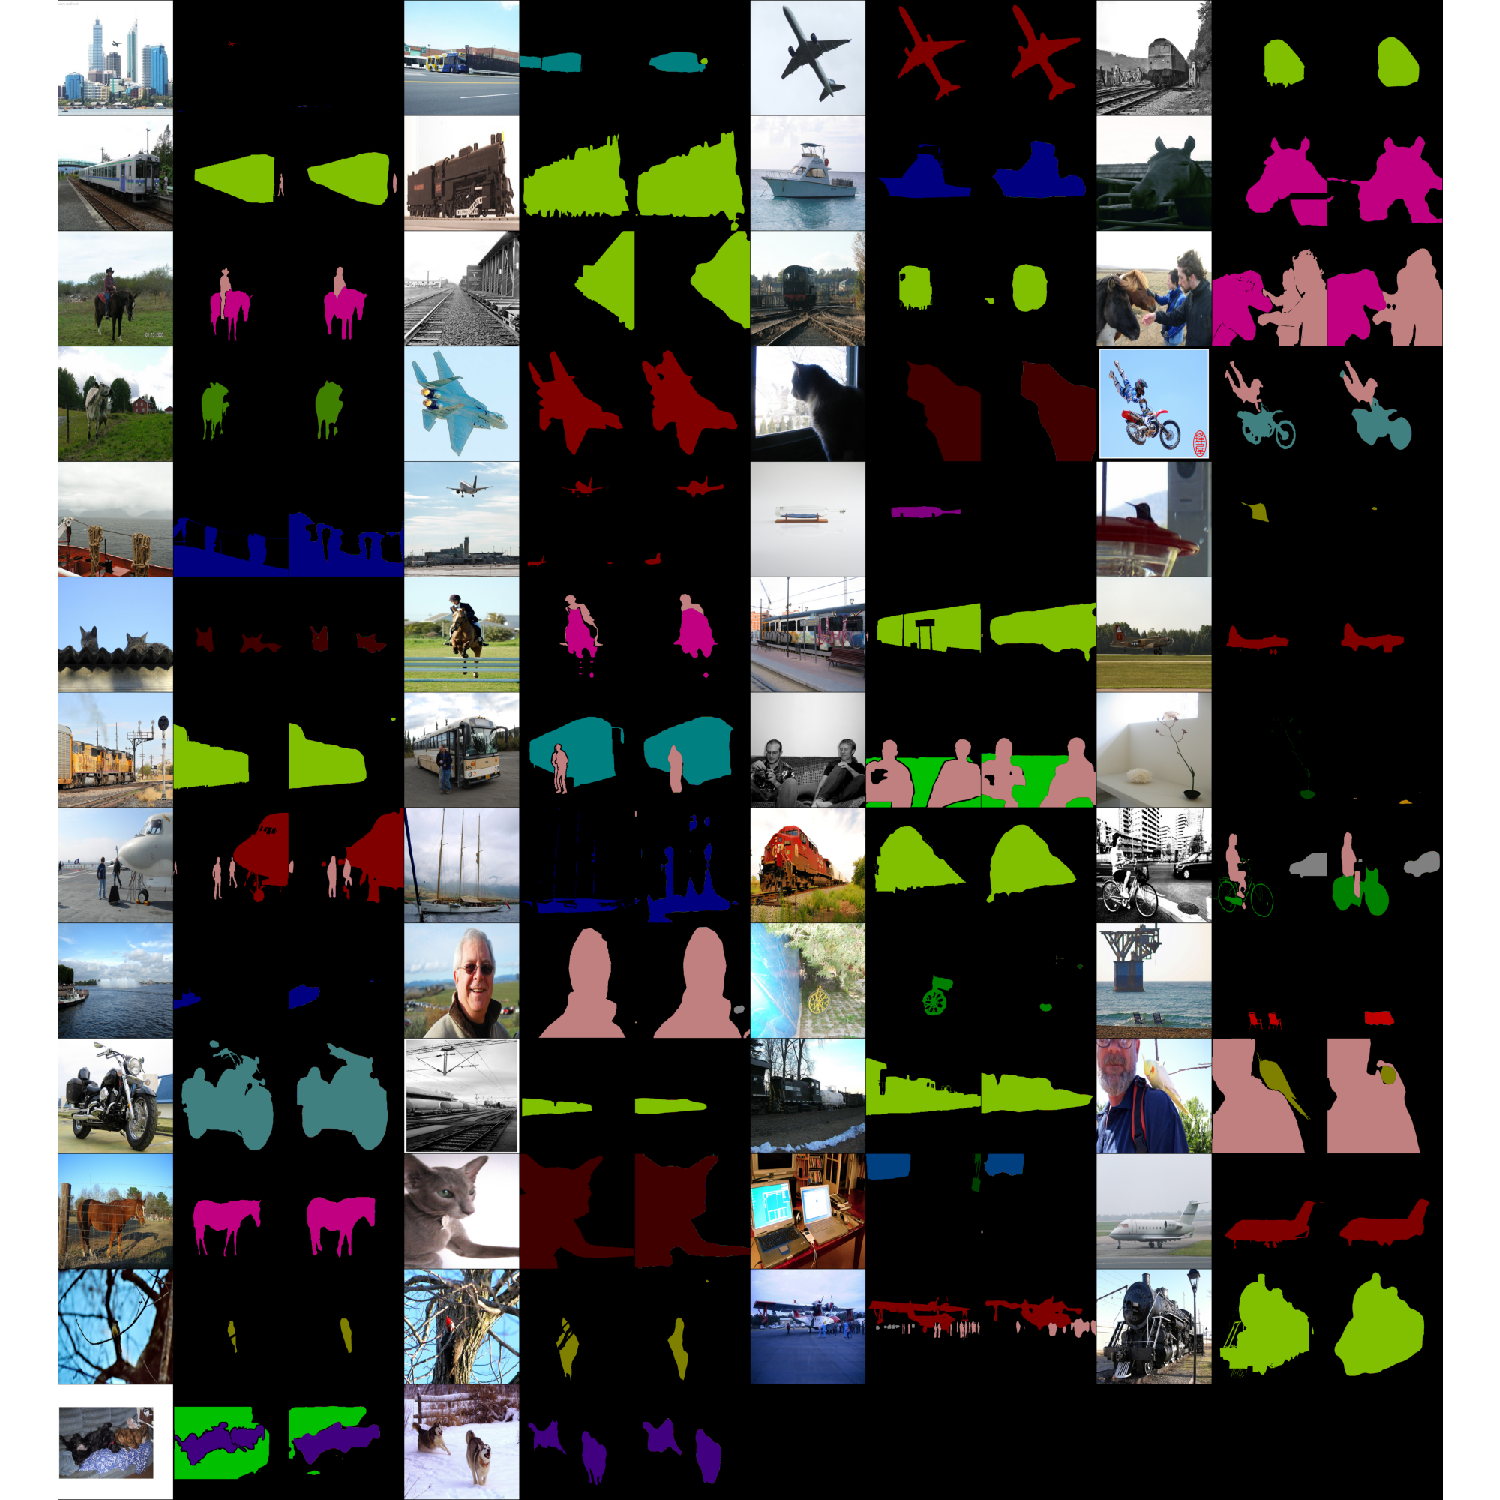
\includegraphics[width=\textwidth]{figures/dsvdd_k50_samples_s.pdf}
%   \caption{Random samples from Top-K=50 DSVDD rankings. The columns (repeated) show input image, ground truth segmentations, and model predictions respectively.  }\label{fig:dsvdd_samples_k50}
% \end{figure*}
